\documentclass{beamer}
\usepackage[utf8]{inputenc}

\usetheme{Madrid}
\usecolortheme{default}
\usepackage{amsmath,amssymb,amsfonts,amsthm}
\usepackage{txfonts}
\usepackage{multicol}
\usepackage{tkz-euclide}
\usepackage{listings}
\usepackage{adjustbox}
\usepackage{array}
\usepackage{tabularx}
\usepackage{gvv}
\usepackage{lmodern}
\usepackage{circuitikz}
\usepackage{tikz}
\usepackage{graphicx}
\usepackage{hyperref}

\setbeamertemplate{page number in head/foot}[totalframenumber]

\usepackage{tcolorbox}
\tcbuselibrary{minted,breakable,xparse,skins}



\definecolor{bg}{gray}{0.95}
\DeclareTCBListing{mintedbox}{O{}m!O{}}{%
  breakable=true,
  listing engine=minted,
  listing only,
  minted language=#2,
  minted style=default,
  minted options={%
    linenos,
    gobble=0,
    breaklines=true,
    breakafter=,,
    fontsize=\small,
    numbersep=8pt,
    #1},
  boxsep=0pt,
  left skip=0pt,
  right skip=0pt,
  left=25pt,
  right=0pt,
  top=3pt,
  bottom=3pt,
  arc=5pt,
  leftrule=0pt,
  rightrule=0pt,
  bottomrule=2pt,
  toprule=2pt,
  colback=bg,
  colframe=orange!70,
  enhanced,
  overlay={%
    \begin{tcbclipinterior}
    \fill[orange!20!white] (frame.south west) rectangle ([xshift=20pt]frame.north west);
    \end{tcbclipinterior}},
  #3,
}
\lstset{
    language=C,
    basicstyle=\ttfamily\small,
    keywordstyle=\color{blue},
    stringstyle=\color{orange},
    commentstyle=\color{green!60!black},
    numbers=left,
    numberstyle=\tiny\color{gray},
    breaklines=true,
    showstringspaces=false,
}
%------------------------------------------------------------
%This block of code defines the information to appear in the
%Title page
\title %optional
{7.4.11}
\date{October 1, 2025}
%\subtitle{A short story}

\author % (optional)
{Aditya Appana - EE25BTECH11004}



\begin{document}


\frame{\titlepage}
\begin{frame}{Question}
If the chord $y = mx + 1$ of the circle $x^2 + y^2 = 1$ subtends an angle of measure $45\degree$
at the major segment of the circle then the value of $m$ is
\begin{enumerate}
\begin{multicols}{4}
    \item $2 \pm \sqrt{2}$
    \item $-2 \pm \sqrt{2}$
    \item $-1 \pm \sqrt{2}$
    \item none of these
    
    \end{multicols}
\end{enumerate}\end{frame}



\begin{frame}[fragile]
    \frametitle{Solution}
The given line subtends an angle $45\degree$ at the major segment of the circle. Therefore, it will subtend $2\times 45\degree = 90\degree$ at the centre of the circle.\vspace{0.6cm}\\
The line $y = mx + 1$ can be expressed as:
\begin{align}
    \myvec{m\\-1}^T\vec{x} + 1 =0
\end{align}\\
This line always passes through $\myvec{0\\1}$, which lies on the circle $x^2 + y^2 = 1$ (since $0^2 + 1^2 = 1$). Therefore one point of intersection is $\myvec{0\\1}$.\vspace{0.6cm}\\
Let the other point of intersection be $\vec{P}$. $\vec{P}$ will be a $\pm90\degree$ rotation of $\myvec{0\\1}$ about the origin.
\end{frame}


\begin{frame}[fragile]
    \frametitle{Solution}
The rotation matrix is:
\begin{align}
\myvec{\cos\theta & \sin\theta \\ -\sin\theta & \cos\theta}.
\end{align}\\
Therefore:
\begin{align}
\vec{P}= \myvec{0\\1}\myvec{\cos(\pm 90\degree) & \sin(\pm90\degree) \\ -\sin(\pm90\degree) & \cos(\pm90\degree)}\\
\vec{P} = \myvec{1\\0} \text{ or } \myvec{-1\\0}
\end{align}
\end{frame}

\begin{frame}[fragile]
    \frametitle{Solution}
\begin{align}
\text{If } \vec{P} = \myvec{1\\0}, m = \frac{0-1}{1-0} = -1   \\
\text{If } \vec{P} = \myvec{-1\\0}, m = \frac{0-1}{-1-0} = 1 \\
m = \pm1
\end{align}
Therefore, \textbf{d)} is the correct answer.
\end{frame}

\begin{frame}[fragile]
    \frametitle{Python, C, Python+C Codes}

\href{https://github.com/AdityaAppana/ee1030-2025/tree/67c35d20c81e9b8d36b9eddc6f9cb710d1aedc9a/ee25btech11004/matgeo/7.4.11/Codes}{codes permalink}

\end{frame}

\begin{frame}
\frametitle{Plot}
\begin{figure}[H]
    \centering
    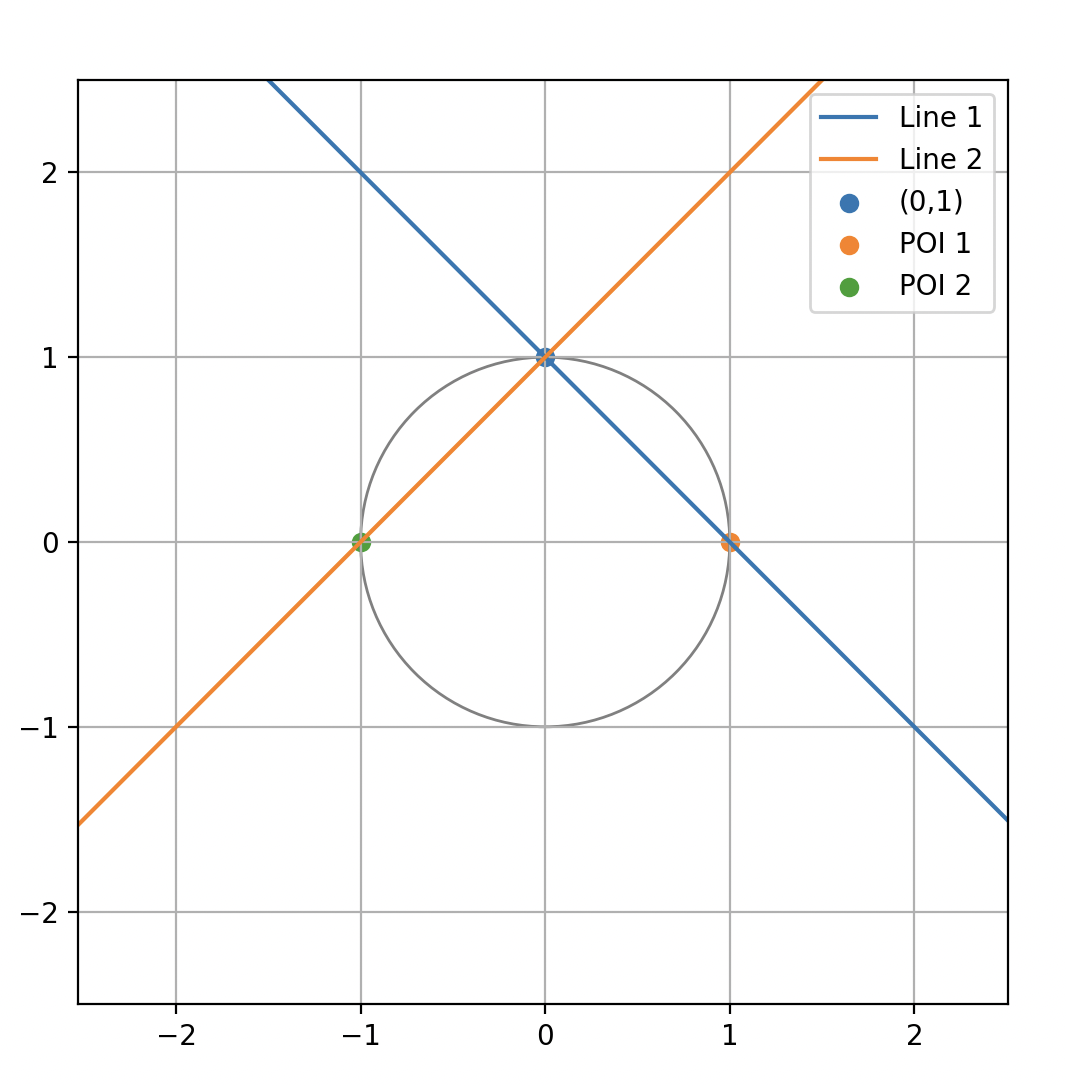
\includegraphics[width=0.6\columnwidth]{Figs/7411.png}
    \caption{Plot}
    \label{fig:placeholder}
\end{figure}

\end{frame}



\end{document}